\documentclass{article}
\usepackage[utf8]{inputenc}
\usepackage[a4paper, total={7in, 10in}]{geometry}
\usepackage{braket}
\usepackage{xcolor}
\usepackage{amsmath}
\usepackage{amssymb}
\usepackage{amsfonts}
\usepackage{graphicx}
\usepackage{svg}
\usepackage{float}
\usepackage{tikz}
\usepackage[ruled,vlined]{algorithm2e}
\usepackage{multicol}
\usepackage[backend=biber,style=alphabetic,sorting=ynt]{biblatex}
\usepackage{xcolor}
%\addbibresource{sample.bib} %Import the bibliography file

\newcommand{\commentt}[1]{\textcolor{blue}{ \textbf{[COMMENT]} #1}}
\newcommand{\ctt}[1]{\commentt{#1}}
\newcommand{\prb}[1]{ \mathbf{Pr} \left[ {#1} \right]}
\newcommand{\onotation}[1]{\(\mathcal{O} \left( {#1}  \right) \)}
\newcommand{\ona}[1]{\onotation{#1}}
\newcommand{\PSI}{{\ket{\psi}}}
\newcommand{\LESn}{\ket{\psi_n}}
\newcommand{\LESa}{\ket{\phi_n}}
\newcommand{\LESs}{\frac{1}{\sqrt{n}}\sum_{i}{\ket{\left(0^{i}10^{n-i}\right)^{n}}}}
\newcommand{\Hn}{\mathcal{H}_{n}}
\newcommand{\Ep}{\frac{1}{\sqrt{2^n}}\sum^{2^n}_{x}{ \ket{xx}}}
\newcommand{\HON}{\ket{\psi_{\text{honest}}}}
\newcommand{\Lemma}{\paragraph{Lemma.}}


\setlength{\columnsep}{0.6cm}

\newcommand{\Gz}{ G_{z}^{\delta} } 

\begin{document}

\title{Quantum LTC With Positive Rate}
\author{David Ponarovsky}
\maketitle
\begin{multicols*}{2}
\newcommand{ \Hw }{ \delta\Delta -\Delta^{\frac{1}{2}-\varepsilon}/\delta  }
	\newcommand{ \Nw }{ \Delta^{\frac{3}{2}-\varepsilon}} 
	  \newcommand{ \Gu } { \Gamma^{\cup} }
	  \newcommand{ \Guq } { \Gamma^{\cup, \square} }

    	\newcommand{ \Gsa } {\Gamma_{\square_{1}} }
	\newcommand{ \Gsah } { \Gamma_{\square_{1}}^{h}} 
	\newcommand{ \Gsb } {\Gamma_{\square_{2}} }
	\newcommand{ \Gsbh } {\Gamma_{\square_{2}}^{h} }
	\newcommand{ \Gssh } { \Gamma_{\square \square }^{h}}
        \newcommand{ \Aa } { C_{A_{1}}}  
	\newcommand{ \Ab } { C_{A_{2}}}
	\newcommand{ \Ac } { C_{A_{3}}}
	\newcommand{ \Ad } { C_{A_{4}}}
	\newcommand{ \Aab } { \Aa \otimes \Ab } 
	\newcommand{ \Acd } { \Ac \otimes \Ad } 
	\newcommand{ \Aac } { \Aa \otimes \Ac }
	\newcommand{ \Aabc } { \Aa \otimes \Ab \otimes \Ac }
	\newcommand{ \Aabcd } { \Aa \otimes \Ab \otimes \Ac \otimes \Ad }
	\newcommand{ \Aabp } { \Aa^{\perp} \otimes \Ab^{\perp} } 
	\newcommand{ \Aacp } { \Aa^{\perp} \otimes \Ac^{\perp} }
	\newcommand{ \Acdp } { \Ac^{\perp} \otimes \Ad^{\perp} }
	\newcommand{ \Aabcdp } { \Aabp \otimes \Acdp }
	\newcommand{ \Aabcp } { \Aa^{\perp} \otimes \Ab^{\perp} \otimes \Ac^{\perp} }
	\newcommand{ \Aabpp } { \left( \Aabp \right)^\perp } 
	\newcommand{ \Acdpp } { \left( \Acdp \right)^\perp } 
	\newcommand{ \Aacpp } { \left( \Aacp \right)^\perp }
	\newcommand{ \Aabcpp } { \left( \Aabcp \right)^\perp }
	\newcommand{ \Aabcdpp } { \Aabpp \otimes \Acdpp  }
	\newcommand{ \App} { \left(\Aabcdpp\right)^{\perp} } 
	\newcommand{ \Aabcdnp } { \left( \Aa \otimes \Ab  \right)^{\perp} \otimes  \left( \Ac \otimes \Ad  \right)^{\perp }}
	\newcommand{ \YY } {  y_{1}y_{2}^{\top} }
	\newcommand{ \ZZ } {  z_{1}z_{2}^{\top} } 
	\newcommand{ \TT } { \tilde{\tau}}
	\newcommand{\EST}{E\left( S,T \right)_{\Gssh} }
	\newcommand{\ESTs}{E\left( S,T \right)_{\text{step}}}
	\newcommand{\BGS}{$( \gamma,\delta,\tilde{\delta})$-BGS }

\paragraph{Tasks.}
	\begin{enumerate}
	  \item Prove that the construction indeed yields a square complex. (The gentle point is to formalize a general TNC property).  
	  \item Prove that $C_{x}$ and $C_{z}$ are indeed CSS pair. Its not so clear how to show that. We hope to prove that either we can choose as generator the forth tensor power product or at least that the generators cubics corresponded to edges in the original graph ( i.e $ \left( g \sim ag  \right) $ edge) share structure (that enforce meeting between duals).
	    % key here is to show that we can choose the genertors to be the matrix $ \Ac \otimes \Ad $   
	  \item Prove a Lemma 1 analogy. And while do so, understand what are the properties we should require from the small code.  
	    (i.e w-robustness and p-resistance for puncturing). 
	    (Make the requirement changes for the new 4D complex with minimal erases, as possible).
	proof. 
	  \item Show that we could actually choose such $\left\{ A \right\}_{i}$ and the matched small codes. (Last priority.) 
	  \item Write a program which plot small complex in a small scale for getting more intuition.  
	\end{enumerate}
	\section{Existance Of 4D Robustness (Small) Codes.} 
	\paragraph{Defintion.} Let $C$ be a linear binary code in $\mathbb{F}^{\Delta}_{2}$. We will say that $C$ has the $\left( \gamma,\delta, \tilde{\delta} \right)-$\textit{Base Generators Set} property if $C$ is spanned by the vectors $V = \left\{v_{0},v_{1},v_{2},\dots v_{m}  \right\} $ such that the weight of any $v_{i}\in V$ is at least $\delta\Delta$ and at most $\tilde{\delta}$. Farthmore for any $j \in [\Delta]$ at most $\gamma\Delta$ vectors from $V$ has the $j$'th bit turn on. Namly:
	\begin{equation*}
	  \begin{split}
	    & | \left\{ v_{i}; v_{i}\in V , \left( v_{i} \right)_{j} = 1  \right\} | \le \gamma\Delta \ \ \ \left( \forall j \in \left[ \Delta \right] \right)
	  \end{split}
	\end{equation*} In adition we will abuse trimonalgy and call $V$ the base of $C$.  
	\paragraph{Robusntess Lemma.} Let $C_{A}$ and $C_{B}$ be codes in $\mathbb{F}^{\Delta}_{2}$ and let $\gamma,\delta$ be constants such $0 < \frac{3}{2}\gamma < \delta < 1$. Assume that both codes above have the $\left( \gamma,\delta \right)-$\textit{Base Generators Set} property. Then any codeword $x\in \Aabpp$ is supported on at most $\frac{|x|}{\Delta\left( \delta-\frac{3}{2}\gamma \right)} $ rows and colomns.     

	\textbf{Proof.} Denote by $\left\{ e_{i} \right\}$ the standard base and by $ V = \left\{v_{0},v_{1},v_{2},\dots v_{m}  \right\} $ the base of $\Aa$ and simelarly let $U = \left\{u_{0},u_{1},u_{2},\dots u_{m}   \right\} $ be the base of $\Ab$. 
	Remind that the dual tensor of $\Aabpp$ is spanned by the products $ \left\{ e_{i}\otimes v_{j} \right\} $ and $\left\{ u_{i}\otimes e_{j} \right\}$ we will call the vectors which are coresponded to $\mathbb{F}^{\Delta} \otimes \Ab$ 'right products' and similary we will give the name 'left products' to the vectors which spans $\Aa \otimes \mathbb{F}^{\Delta}$. 
	Let us write $x$ as formal sumtion. And let $\#_{A},\#_{B} $ be the set of of right and left products in that sumtion. Then by taking in account only the pairs intersection we have that:  
	\begin{equation*}
	  \begin{split}
	    |x| & \ge \sum_{\xi \in \#_{A} }{w\left( \xi \right)} +   \sum_{\xi \in \#_{B} }{w\left( \xi \right)}  -{ \sum}_{\xi, \eta \in  \#_{A} \cup  \#_{B}}{ w\left( \xi \cap \eta \right) }\\
	    & \ge \left( \#_{A} + \#_{B} \right)\delta\Delta - { \sum}_{\xi, \eta \in  \#_{A} \cup  \#_{B}}{ w\left( \xi \cap \eta \right) } \\ 
	  \end{split}
	\end{equation*} Split to cases, first case, $\xi,\eta$ are both right (or left products). In the case we are intersted in the intersection of: 
	\begin{equation*}
	  \begin{split}
	    e_{i}\otimes v_{t} \cap e_{j} \otimes v_{s} = \begin{cases}
		        0 & i \neq j \\
			v_{t} \cap v_{s}  &\text{else}
        \end{cases}
	  \end{split}
	\end{equation*} By the fact that there is at most $\gamma\Delta$ vectors $v\in V$ which their $s$-cordinate is not zero we get that the total contribution of such intersections is bounded from above by $\#_{A}\gamma\Delta + \#_{B}\gamma\Delta $.
	In the seconed case consider the intersection of left and right products. in that case we have: 
	\begin{equation*}
	  \begin{split}
	    e_{i}\otimes v_{t} \cap  u_{s} \otimes e_{j}= \begin{cases}
	      0 & \left( v_{t} \right)_{j} = 0 \text{ or } \left( u_{s} \right)_{i} = 0 \\
			1  &\text{otherwise}
        \end{cases}
	  \end{split}
	\end{equation*} \color{red} Taking in acount higher momuntens \textbf{only} in the second case is still preserving the inequality direction? For now assume also that $C$ has maximal weight of $\tilde{\delta} = \Theta\left(\frac{1}{\Delta} \right)$. \color{black} 
	By the assumption that $C$ has maximal weight of $\tilde{\delta}$ we get that the contribuation of the second case is bounded by
	\begin{equation*}
	  \begin{split}
	    & \frac{1}{2}\left( \#_{A}+\#_{B} \right)\gamma\Delta\tilde{\delta}\Delta \\ &  \Rightarrow \#_{A},\#_{B} \le \frac{|x|}{\Delta\delta - \Delta\gamma - \frac{1}{2}\gamma\tilde{\delta}\Delta^{2}} 
	  \end{split}
	\end{equation*}
	\paragraph{Definition.} Let $C$ be a code. We will say that a code $C^{\prime}$ is obtained by $p$-pancurting from $C$ if there exists a set of indecis $A$ at size $ |A| \in [ \Delta - p , \Delta ] $  such that for any codeword $c^{\prime}$ there exists codeword $c \in C $ such that for any $ i \in \left[ |A|  \right] $ it holds that $c^{\prime}_{A_{i}} = c_{i}$.    
	\paragraph{Lemma. $p$-resistence conserve $\gamma$-property. } Let $C$ be a code wich has the $\left( \gamma,\delta, \tilde{\delta} \right)-$\textit{Base Generators Set} property. 
	Then any code $C^{\prime}$ obtained from $C$ by $p$ panucturing has the $\left( \gamma,\delta - p, \tilde{\delta} \right)-$\textit{Base Generators Set} property.
	
	\textbf{Proof.} The proof is trival. 
	%\paragraph{Graph Represantion Of The Base. } Def. 
	\paragraph{The Dual Tensors Have $\left( \gamma,\delta \right)-$generators base set.} Let $\Aa$ and $\Ab$ be codes that have the $\left( \gamma,\delta, \tilde{\delta} \right)-$\textit{Base Generators Set} property. Then the dual tensor of the code $\Aabpp$ has $\left( 2\gamma/\Delta,\delta/\Delta, \tilde{\delta}/\Delta \right)-$\textit{Base Generators Set} property.

	\textbf{Proof.} The proof is trival. 
	\paragraph{Existance Of \BGS Codes}. We will now show that the LTC codes of Levarier and Zemor has the \BGS property. Let $\mathcal{C}$ be the $\left[n, k\ge \left( 2\rho^2-1 \right)n, d\ge \beta^{2}\left( \beta - \lambda/\Delta \right)n \right]$ LTC code defined in \color{blue} cite\color{black}. And recall that $\mathcal{C} \subset C^{\perp}_{z}$. The distance of their CSS code is greter than $\tilde{\delta}n=\left( \beta / 4\Delta^{3/2+\varepsilon} \right)n $. \\
	By defination the distance of the CSS code is the weight of the smallest codeword in $C_{x}$ which is not in $C^{\perp}_{z}$. Hence, the codewords of $\mathcal{C}$ are at weight no more the the maximal weight of codeword of  $C^{\perp}_{z}$ which is at most $\tilde{\delta}n$. \\
	Hence it's left to show that we could pick a base which has no more than $m$ vectors sharing the same bit. By Theorem 1 in \color{blue}cite\color{black} the set of codewords which entirly supported on the neighbourhood of negative codewords spans the the codeword of $C^{\perp}_{z}$ and any vecor set which spans $\mathcal{C}$ could represnted as linear transforamrion over the any set which sapns $C^{\perp}_{z}$.
	Denote by $U = \{u_{0},u_{1},u_{2},\dots u_{\rho} \}$ the set which spans $\mathcal{C}$, and assume that $U$ is also the base, namly $\log \dim U = \log \dim \mathcal{C} = \rho n $. And by $V = \{v_{0},v_{1},v_{2},\dots v_{q}  \} $ the set which spans $C_{z}^{\perp}$ and also $v_{i}$ assosiate with setting some codeward in $\Aab$ over the some vertex. 

	Let $A\in \mathbb{F}^{\rho \times q}_{2}$ be the matrix such $AV = U$.
	%$C_{ Take the base,   
	
 \paragraph{The Construction.} Fix primes $q,p_0,p_2,p_3,p_4$ such that each of them has $1 $ residue mode $4$. Let $A_{1},A_{2},A_{3},A_{4}$ be a different generators sets of $ \mathbf{PGL}(2 , \mathbb{Z} / q\mathbb{Z} )  $ 
  obtained by taking the solutions for $a_{0}^{2} + a_{1}^{2} +a_{2}^{2} +a_{3}^{2} = p_i $ such that the pairs $A_{1},A_{2}$ and $A_{3},A_{4}$ satisfy the 
  TNC constraint and also they all satisfy that constraint together, manly for any $g \in \mathbf{PGL}$  and $a_{1}\in A_{1}, a_{2} \in A_{2}, a_{3} \in A_{3}, a_{4} \in A_{4}$ we have that $ g \neq a_{3}a_{1}ga_{2}a_{4}$. 
  
  For any $h \in \mathbb{Z}_{3}^{2} $ define the groups $G^{h}, H^{h}$ to be: 
  \begin{equation*}
    \begin{split}
      H^{h} &=  h + \mathbb{Z}_{3}^{2}\cap \braket{ \left( 1,1 \right)} \\
      G^{h} &=  \mathbf{PGL}  \times H^{h} 
    	\end{split}
\end{equation*} 
  Then consider the graphs:   
  \begin{equation*}
    \begin{split}
      %\Gamma_{1}  &= Cay_{3}\left(  G, A_{1} \right)\times_{G} Cay_{3}\left(  G, A_{2} \right) \\
      %\Gamma_{2}  &= Cay_{3}\left(  G, A_{3} \right)\times_{G} Cay_{3}\left(  G, A_{4} \right) \\
      \Gamma_{\square_{1}}^{h} &= \bigg( G^{h}, \bigg{\{} \left( \left(g, h_{1} \right),\left(  agb,h_{1} + \left( 1,1 \right)  \right)\right) :  \\ 
      &  a \in A_{1}, b \in A_{2}, h_{1} \in H^{h}  \bigg{\}}  \bigg) \\
      \Gamma_{\square_{2}}^{h} &= \bigg( G^{h}, \bigg{\{} \left( \left(g, h_{1} \right),\left(  cgd,h_{1} + \left( 1,1 \right)  \right)\right) :  \\ 
      &  c \in A_{3}, d \in A_{4}, h_{1} \in H^{h}  \bigg{\}}  \bigg) \\
      \Gamma_{\square \square}^{h} &= \bigg( G^{h}, \bigg{\{} \left(\left(g, h_{1} \right),\left(  cagbd, h_{1} + \left( 2,2 \right)  \right)\right), \left( g, acgdb \right) :\\
      & a \in A_{1}, b \in A_{2}, c \in A_{3}, d \in A_{4}, h_{1}\in H^{h} \bigg{\}}  \bigg) 
    \end{split}
  \end{equation*}
   Then define the codes:
	\begin{equation*}
	  \begin{split}
	    C_{z} & = \mathcal{T}\left( \Gssh,  \Aabcdnp  \right) \\
	    C_{x} &=  \mathcal{T}\left(  \Gssh, \Aabcdpp  \right) \\
	    C_{w} &=  \mathcal{T}\left( \Gssh , \App \right)   
	  \end{split}
	\end{equation*}
	Notice that that $C_{x}$ could be viewed as the classical LTC code in Levarier and Zemor construction by treating the tensor product as standing alone small code. \ctt{ Task 1. }  

	 
	\begin{figure}[H]
	%\label{zafig:square}
	  \begin{center}
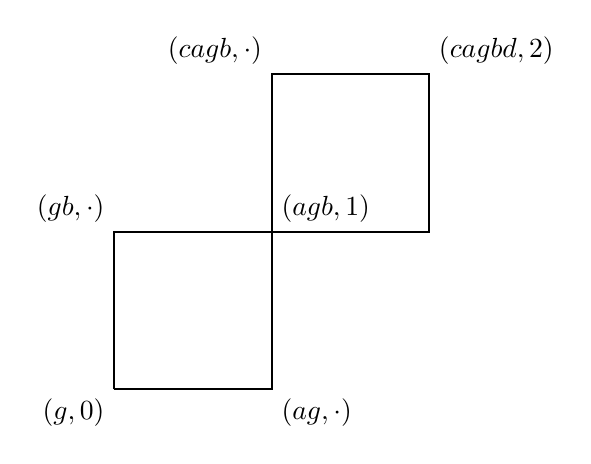
\begin{tikzpicture}
  \draw[thick] (0,0) -- (0,2) -- (2,2) -- (2,4) -- (4,4) -- (4,2) -- (2,2) -- (2,0) -- (0,0);
\node[below left] at (0,0) {$ (g,0)$};
\node[above left] at (0,2) {$ (gb,\cdot)$};
\node[above right] at (2,2) {$ (agb,1)$};
\node[below right] at (2,0) {$ (ag,\cdot)$};
\node[above left] at (2,4) {$ (cagb,\cdot)$};
\node[above right] at (4,4) {$ (cagbd,2)$};

\end{tikzpicture}
\end{center}
\caption{Square of the complex, with edges $(g,ag), (agb, gb) \in E_A,
(g,gb), (agb, ag) \in E_B.$ \label{fig:square}
}
\end{figure}


%\paragraph{Lemma 1.} Fix a vertex $g$ and assume that the local views $c_1,c_2$ that lay over the graphs $\Gsa, \Gsb$ belongs to the dual tensors $\Aabpp, \Aacpp$. And inaddtion $ 1^{\Delta} \in \Aa $ then 
%      \begin{equation*}
%      \phi_{g}\left( c_1, c_2 \right) \in \Aabcpp
%    \end{equation*}
%    \paragraph{Proof.} The case where $c_{1} \in \mathbb{F}^{A_{1}} \otimes \Ab$ or $c_{2} \in \mathbb{F}^{A_{1}} \otimes \Ac $ is trival. Suppose that both $ c_{1} \in \Aa \otimes \mathbb{F}^{A_{2}}$ and $ c_{2} \in \Aa \otimes \mathbb{F}^{A_{3}}$. And consider by $h$ arbirary check of $\Aa$.Then: 
%    \begin{equation*}
%      \begin{split}
%	\braket{h_{bc}, \phi_{g} \left( c_1, c_2 \right)  } & \ \ \ \ \ = \sum_{a}{h_{a}c_{abc}} = 
	  %\sum_{a}{h_{a}c_{1_{ab}}c_{2_{ac}}} = \\ 
	  %&\overset{\text{ for  } y,z\in \Aa}{\overbrace{=}}  \sum_{a} h_{a}z_{a}y_{a} \\ 
	  %&\ \ \ \ \ = |h| -  \sum_{a} {h_{a} \left( \overline{ z_{a}y_{a}}  \right)} \\
	  %&\ \ \ \ \ = |h| -  \sum_{a} {h_{a} \left( z_{a} + y_{a}  \right)} \\  
	  %&\ \ \ \ \ = |h| +  \sum_{a} {h_{a} \left( z_{a} + y_{a}  \right)} \\ 
	  %&\ \ \ \ \ =  \sum_{a} {h_{a} \left( 1^{\Delta} + z_{a} + y_{a}  \right)} 
      %\end{split}
    %\end{equation*}
    %But $1^{\Delta} \in \Aa$ and therfore the $ \braket{h, 1^{\Delta} + z + y} = 0 $. Or in other words the words that lay over the row obtained by fixing $bc$-row is in $ C_{A_{1}}$. Hence $\phi \left( c_{1}, c_{2} \right) \in C_{A_{1}}\otimes \mathbb{F}^{A_{2}} \otimes \mathbb{F}^{A_{3}} \subset \Aabcpp$.   
%
    	%\paragraph{What We Currently Have.} Given a candidate for a codeword $c$ we could check efficiently if $c\in C_{z}^\perp$.  
	%Additionally summing up the local correction of each vertex in $C_{x}$ yields a codeword in $C_{w}$. Now we would want to show 
	%something similar to property 1 in Levarier and Zemor which imply that any codeword of $C_{w}$ with weigh beneath 
	%a linear threshold $\eta n $ must to be also in $C_{X}$. (And therefore we can reject candidates with high weight). 
	%%(And maybe we would also say something about the gap between the this minimal weight of $C_{w}/C_{x}$. 
%
	%Assume that we have succeed to do so, Then the testing protocol will be looked as follow, 
	%first we check that the candidate is not in $C_{z}^\perp$ and then we check that is indeed in $C_{x}$. And repeat again 
	%in the phase base. Then there are constants $\kappa_1, \kappa_2$ 
	%\begin{equation*}
	  %\begin{split}
	    %\text{accept} & \sim \kappa_1 \cdot  d\left( c,C_{z}^\perp \right)  \\ 
	    %& +  \left[ 1 -  \kappa_1 \cdot  d\left( c,C_{z}^\perp \right)\right] \kappa_{2} d\left( c, C_{x} \right) \\
	    %\text{reject} & \sim  \left[ 1 -  \kappa_1 \cdot  d\left( c,C_{z}^\perp \right)\right] \\ 
	    %& +\kappa_1 \cdot  d\left( c,C_{z}^\perp \right) \cdot \left[ 1 - \kappa_{2} d\left( c, C_{x} \right) \right] 
	  %\end{split}
	%\end{equation*}
	%\paragraph{Disclaimer.} The use of the $\sim$ was  made by purpose. The above should be formalize by inequalities. (And this also make another problem as 
	%the term $ 1 - \kappa_{1} \cdot d\left(  \right) $ is in the opposite direction). 
	%\paragraph{The zHard Part.} It seems (at least for now) that the hard part is to find an analog for Lemma 1 in Levrier-Zemor, Which can formalize 
	%as follow: Consider a codeword $c \in C_{w}$ such that $|c| \le \eta n $ then we could always find a vertex in $\Gamma_{\square_{1}} $
	%and a local codeword $\xi \in C_{A_1} \otimes c_{A_2} $ on his support such that $|c + \xi| < |c| $.     
      

		% be a codeword with weight less then $\alpha n$.

\paragraph{Lemma 1} \textit{ The pair $C_{x},C_{z}$ defined above is CSS code. } 

\textbf{Proof.} Let $c^{\left( 1 \right)}, c^{\left( 2 \right)}$ be codewords in $C_{x}$ and $C_{z}$ then: 

\begin{equation*}
  \begin{split}
    \braket{c^{\left( 1 \right)}, c^{\left( 2 \right)}} &= \sum_{\text{plaquettes}}c^{\left( 1 \right)}_{i} c^{\left( 2 \right)}_{i}= \sum_{\text{plaquettes}}c^{\left( 1 \right)}_{gabcd} c^{\left( 2 \right)}_{gabcd} \\ 
    &= \sum_{cd}{\sum_{gab}{ c^{\left( 1 \right)}_{gabcd} c^{\left( 2 \right)}_{gabcd} }} 
  \end{split}
\end{equation*}
By the fact that for any fixed $c,d$ we have that the induced words are codewords of the orignal codes (from Zemor and Levarier) the product above is zeroed.  
	\paragraph{Plaquettes Expansion.} Let, $S , T$ be vertices subsets of $G^{h}$ and Let $S^{\star}$ be the vertices which can be reached from $S$ trough edges from $\Gsah$. By regularity it's clear that $S^{\star}\le \Delta^{2}|S|$. In addition, by the fact that $G^{h}$ is a group, we have that $agb = ag^{\prime}b$ if and only if $g = g^{\prime}$. 
	Therefore we could derive a lowerbound on the size of $S^{\star}$ by fixing $a,b$ and consider the vertices corresponded to $aSb \subset S^{\star}$.    
	Then by the mixing expansion lemma we get: 
	\begin{equation*}
	  \begin{split}
	  \EST &= E\left( S^{\star}, T  \right)_{\Gsah} \\
	|\EST| &\le \frac{\Delta^{2}}{n}\Delta^{2}|S||T| + \lambda_{\Gsbh}\Delta\sqrt{|S||T|} \\ 
      |\EST| &\ge \frac{\Delta^{2}}{n}|S||T| - \lambda_{\Gsbh}\sqrt{|S||T|}  
	  \end{split}
	\end{equation*}
	\paragraph{Step-Edges Expansion.} Let us define a step-edge to be a concation of $e_{1},e_{2}$ edges in $\Gsah, \Gsbh$ such that $e_{1},e_{2}$ are adjacent in the union of $\Gsah, \Gsbh$ and they both either left or right edges. 
	Now consider again two vertices subsets $S$ and $T$ and denote by $ \ESTs $ the cut contains the step-edges between $T$ and $S$.
	Consider now subsets $S^{\star}_{L}$ and $S^{\star}_{R}$ which are the vertices which can be reach from $S$ trough left, right edges. And notice that each step-edge is a path compused by an source vertex from $S$, an intermdiate vertex from $S^{\star}_{L}$ or $S^{\star}_{R}$ and a target vertex from $T$. 

	In addition, by regularity the size of $S^{\star}_{L}$ is at most $\Delta|S|$.
	And again by the fact that the edges are coressponded to Group generators, $S^{\star}_{L}$ can be bounded from below by considering the multiplication of $S$ by single generator.    
	

	Hence by applaing the Mixing Lemma we have: 
		\begin{equation*}
	  \begin{split}
	    \ESTs &= E\left( S^{\star}_{L}, T  \right)_{\cdot} +  E\left( S^{\star}_{R}, T  \right)_{\cdot} \\
	|\ESTs| &\le \frac{2\Delta}{n}\Delta|S||T| + 2\lambda\sqrt{\Delta|S||T|} \\ 
      |\ESTs| &\ge \frac{2\Delta}{n}|S||T| - 2\lambda\sqrt{|S||T|}  
	  \end{split}
	\end{equation*}



\paragraph{Dense Normal Net Counting} Let us call the normal vertices the vertices with degree less then $\xi$ in $\Guq = \Gamma_{\square, 1}^{x} \cup \Gamma_{\square, 2}^{x}$. 
And Let us say that a step-edge is an heavy edge if it incidents to at least $\eta$ plaquettes.

Let $ T$ be set of vertices in $V_0$ that are connected to (at least) one normal vertex through a heavy edge.  

    Recall that the distance of the tensor code equal to the   notice that the number of vertices in the induced graph by $x$ is bounded by it's weight:
    $ |S| \le \frac{2|x|}{ \delta^{2}\Delta^{2} }$ 

    By the mixing Lemma we get:  
    \begin{equation*}
      \begin{split}
	| \ESTs | & \ge \eta |T| \\ 
	\Rightarrow  & |T|\left( \eta - \frac{2\Delta^{2}\cdot 2|x|}{n\left( \delta\Delta \right)^{2}}  \right) \le  2 \lambda\sqrt{\Delta|S||T|} 
      \end{split}
    \end{equation*}
    Hence we have that:
    \begin{equation*}
      \begin{split}
	& \sqrt{|T|}\left( \eta - \frac{2\Delta^{2}\cdot 2|x|}{n\left( \delta\Delta \right)^{2}}  \right) \le   2\lambda\sqrt{\Delta|S|} \\ 
	& |T| \le \left( \frac{ 2\lambda\sqrt{\Delta}}{\eta - \frac{4 |x|}{n\ \delta^{2}} } \right)^{2} |S|	
      \end{split}
    \end{equation*}
    Denote by $S_{e}$ the set of vertices in $\Guq$ with degree greater then $\xi$. Then by repeating on the above calculation, while substituting $\Gamma_{i}$ by $\Gamma_{i, \square}$, We obtain that there is $\lambda^{\star}_{2}$ such that:
     \begin{equation*}
      \begin{split}
	| \EST | & \ge \xi |S_{e}| \\ 
	\Rightarrow  & |S_{e}|\left( \xi - \frac{\Delta^{4}\cdot 2|x|}{n\left( \delta\Delta \right)^{2}}  \right) \le   \lambda_{\Gsbh}\Delta\sqrt{|S||S_{e}|} 
      \end{split}
    \end{equation*}
    Hence we have that:
    \begin{equation*}
      \begin{split}
	& \sqrt{|S_{e}|}\left( \xi - \frac{\Delta^{4}\cdot 2|x|}{n\left( \delta\Delta \right)^{2}}  \right) \le   \lambda_{\Gsbh}\Delta\sqrt{|S|} \\ 
	& |S_{e}| \le \left( \frac{ \lambda_{\Gsbh}\Delta}{\xi - \frac{\Delta^{2}\cdot 2|x|}{n\ \delta^{2}} } \right)^{2} |S|	
      \end{split}
    \end{equation*}

   Define $\bar{d}_{T}$ to be the average (over $T$) of heavy edges incident to a vertex of $T$. So 
    \begin{equation*}
      \begin{split}
	\bar{d}_{T} &= \frac{|E\left( T, S / S_{e} \right)|}{T} \ge \frac{|S| - |S_{e}|}{|T|} \\
	& \ge \left( 1 -   \left( \frac{ \lambda_{\Gsbh}\Delta}{\xi - \frac{\Delta^{2}\cdot 2|x|}{n\ \delta^{2}} } \right)^{2}\right) /  
	  \left( \frac{ 2\lambda\sqrt{\Delta}}{\eta - \frac{4 |x|}{n\ \delta^{2}} } \right)^{2}
      \end{split}
    \end{equation*}
    Let us call to the quantity above $2\Delta^{2}\rho$ and denote by $1 - \tau$ the fraction of vertices of $ T $ with step-edges degree less then $\frac{1}{2}2\Delta^{2}\rho$. 
    Then $ \frac{1}{2}2\Delta^{2}\rho \le \bar{d}_{T} \le 2\Delta^{2}\tau + \left( 1 - \tau \right) 2\Delta^{2}\rho  $ 
    $ \Rightarrow \tau \ge \frac{\rho}{2\left( 1 - \rho \right)}\ge \rho/3 $. Namely, at least $\rho/2$ of vertices of $T$ are incident to at least $\frac{1}{2}2\Delta^{2}\rho$ heavy edges. 

    Since each vertex is a source for at most $2\Delta^{2}$ step-edges we get that $|S| - |S_{e}| \le 2\Delta^{2}|T| $. 

    \color{red} mark \color{black} In the other-hand we have shown that 
 \begin{equation*}
   \begin{split}
     |S_{e}| &  \le \left( \frac{ \lambda_{\Gsbh}\Delta}{\xi - \frac{\Delta^{2}\cdot 2|x|}{n\ \delta^{2}} } \right)^{2} |S| \\ &
     \Rightarrow |S| \le \left( 1 - \left( \frac{ \lambda_{\Gsbh}\Delta}{\xi - \frac{\Delta^{2}\cdot 2|x|}{n\ \delta^{2}} } \right)^{2}\right)^{-1}2\Delta^{2}|T| \\
     & = \left( 1 - \theta^2 \right)^{-1} 2 \Delta^{2} |T|
   \end{split}
 \end{equation*}
 And by using again the mixing Lemma we have that: 
 \begin{equation*}
   \begin{split}
     E\left( S_{e},T \right)_{\text{step}} &\le \frac{\theta^2}{1- \theta^2}2\Delta^{2}|T|^2 \frac{2\Delta^{2}}{n} + \lambda\sqrt{\frac{\theta^2}{1- \theta^2}}|T| \\ 
     & \le  \left( \frac{\theta^2}{1- \theta^2}4\Delta^{2} + \lambda\sqrt{\Delta}\sqrt{\frac{\theta^2}{1- \theta^2}}\right)|T| \\ 
%     & \le \left(9\Delta^{2} + \lambda^{\star} \right) |T|
  \end{split}
 \end{equation*}
 Hence at most an $\frac{1}{6}\rho $ proportion of vertices of $T$ are adjacent to more than $\frac{6}{\rho} \left( 4\Delta^{2} + \lambda  \right) $ vertices of $S_{e}$, And at least $\frac{5}{6}\rho$ proportion of $T$ are adjacent to less then $\frac{6}{\rho} \left( 4\Delta^{2} + \lambda  \right) $ . 
 And therefore we have that at least $\frac{1}{6}\rho$ vertices are:
 \begin{enumerate}
   \item Incident to at least $\frac{1}{2}2\Delta^{2}\rho$ heavy edges. 
   \item Adjacent to at most $ \frac{6}{\rho} \left( 4\Delta^{2} + \lambda \sqrt{\Delta}  \right)$ vertices of $S_{e}$.  
 \end{enumerate}
	\paragraph{All The Vertices Are Normal} Define a normal vertex in $ V_{1} $ to be a vertex such his local view (a codeword in a dual tensor code). 
	supported on less then $w = \Delta^\frac{3}{2}$ faces.
	Consider the code $C_{w}$ defined above, and assume in addition that the distance and the rate of 
	the small codes $C_{A_{j}}$, $\delta \Delta$ satisfy the equation $ \left(\Delta r\right)^{4}\left(1 - \color{red}2\color{black}\delta\right) < \frac{1}{2}\delta^{3} $ and also the code $ C_{A_{1}}  $ 
      contains the word $ 1^{\Delta} $.


      Then for any $x \in C_{w}$ such that all the vertices in the induced graphs $\Gamma_{\square_{1}},\Gamma_{\square_{2}}$  by it are normal. 
	Then there exists a vertex $ g \in V_{0} $ and a local codeword $ c \in \Aabc $ supported entirely on the neighborhood of $ g $ such that: 
	$ |x + c| \le |x| $.


	\paragraph{Proof.} Let $g$ be an arbitrary vertex in $V_{0}$ we know by Leverrir and Zemor that the local views of $g$ in  $\Gamma_{\square_{1}},\Gamma_{\square_{2}}$ are $\Delta^{3/2}$ close to 
      $\Aab $ and $ \Aac $ by the $w$-robustness property. 

	So we can represent the locals views on $g$ as the following disjointed vectors, each lays on $\Gamma_{\square_1},\Gamma_{\square_2}$:
	\begin{equation*}
	  \begin{split}
	    y &= y_{1}y_{2}^{\top} + \xi_{y} \\ 
	    z &= z_{1}z_{2}^{\top} + \xi_{z}
	  \end{split}
	\end{equation*}
	such that $ y_{1}y_{2}^{\top} \in \Aab $,  $z_{1}z_{2}^{\top}\in \Aac $ and the $\xi_{y}, \xi_{z} $ are the corresponded errors of the local views from the tensor codes. 
 
	Let $ \{ y_{1}^{j}y_{2}^{i \ \top} \} ,\{ z_{1}^{j}z_{2}^{i \ \top} \}  $ be the bases for $ \Aab $ and $ \Aac $ such that $ y_{1}^{j}, z_{1}^{j} \in \Aa $ and $ y_{2}^{i} \in \Ab, z_{2}^{i} \in \Ac $.  
	And denote by $\alpha_{ij},\beta_{ij} \in \mathbb{F}_2 $ the coefficients of $\YY$ and $\ZZ$. 

	By the fact that $1^\Delta \in \Aa$ we have that for any $i,j$ the vector: 
	\begin{equation*}
	  \begin{split}
	  \bar{y_{1}}^{j}y_{2}^{i \ \top} & =  1^\Delta y_{2}^{i \ \top} \\ 
	    & + y_{1}^{j}y_{2}^{i \ \top} = \left(1^\Delta +  y_{1}^{j} \right)y_{2}^{i \ \top} \\
	    & \in \Aab
	  \end{split}
	\end{equation*}
      And by the same calculation we get also that $ \bar{z_{1}}^{j}z_{2}^{i \ \top} \in \Aac$.

      \paragraph{Claim.} Assume that $ \YY $ and $ \ZZ $ are in the  bases defined above. Let $\tau \in \mathbb{F}_{2}^{A\times B\times C} $ such that $ \tau_{abc} = \left( \YY \right)_{ab}\left( \ZZ \right)_{ac} $ then: 
      \begin{equation*}	
      d\left( \tau, \Aabc \right) \le \left( 1-\delta \right)\Delta^{3}  
      \end{equation*}
      \paragraph{Proof.} First notice that $y_{1a}y_{2b}z_{2c} $ is a valid codeword of $\Aabc$. That because that the projection obtained by 
      fixing any two coordinates yields either a zero or a codeword of one the codes.
      
      Therefore we could consider the following codeword $ \TT_{abc} = \left( y_{1a} + \bar{z}_{1a} \right)y_{2b}y_{2c} $ and bounding the distance of $\tau$ by 
      \begin{equation*}
	\begin{split}
      & d \left( \tau, \Aabc \right)  \le d \left( \tau, \TT \right) \\ 
      & = \sum_{abc}{   \left( y_{1a} + \bar{z}_{1a} \right)y_{2b}y_{2c} \oplus  \left( y_{1a}z_{1a} \right)y_{2b}y_{2c}  } \\
      & =  \sum_{abc}{   \left( y_{1a} + \bar{z}_{1a} \oplus y_{1a}z_{1a}  \right)y_{2b}y_{2c}  } \\
      & \le | \left\{ y_{1a} = 0 \text{ and }  z_{1a} = 0   \right\} | \cdot \Delta^{2} \le \left( 1-\color{red}2\color{black}\delta \right)\Delta^{3} 
	\end{split}
      \end{equation*}

      \paragraph{Claim.} Let $\YY, \ZZ$ be codewords in $\Aab, \Aac$. And let $w$ be the vector define by $w_{abc} = \left( \YY \right)_{ab} \left( \ZZ \right)_{ac} $. Then  
      \begin{equation*}
	d\left(w, \Aabc \right) \le \left( r\Delta \right)^{4}\left( 1 - \delta \right)\Delta^{3} + \Theta \left( \Delta^{2\frac{1}{2}}  \right)
      \end{equation*}

      Consider again the representation of the local view $w$ on the vertex $g$. 
      \begin{equation*}
	\begin{split}
	  & w_{abc} = y_{ab}z_{ac} = \left( \YY + \xi_{y} \right)_{ab}   \left( \ZZ + \xi_{z} \right)_{ac} \\ 
	  & \left( y_{1}y_{2}^{\top}\right)_{ab}\left(z_{1}z_{2}^{\top} \right)_{ac} = 
	  \left( \sum_{ij} { \alpha_{ij} y_{1}^{i}y_{2}^{j  \top}}  \right)_{ab}\left(   \sum_{ij} { \beta_{ij} z_{1}^{i}z_{2}^{j  \top}} \right)_{ac}\\ 
	  &= \sum_{ijlk} { \alpha_{ij}\beta_{lk} y_{1a}^{i}y_{2b}^{j \top}} z_{1a}^{l}z_{2c}^{k \top} \\
	  & \Rightarrow d\left( \sum_{abc} \left( y_{1}y_{2}^{\top}\right)_{ab}\left(z_{1}z_{2}^{\top} \right)_{ac} , \Aabc \right) \\ 
	  & \ \ \ \ \le \left( \Delta r \right)^{4} \left( 1-\delta \right)\Delta^{3} \\ & 
	  %+  \left( \xi_{y} z_{1}z_{2}^\top + \xi_{y}\xi_{z}, \Aabc   \right)  
	\end{split}
      \end{equation*}
      In addition its clear that $ | \sum_{abc}{\xi_{ab}\left( \ZZ + \xi\right)_{ac}} | \le  \sum_{c}\sum_{ab}{|\xi_{ab}|} \le \Delta^{ 2\frac{1}{2}} $. Hence, we have that 
  \begin{equation*}
    \begin{split}
      d\left( w, \Aabc  \right) \le  \left( r\Delta \right)^{4}\left( 1 - \delta \right)\Delta^{3} + \Theta \left( \Delta^{2\frac{1}{2}}  \right)
    \end{split}
  \end{equation*}
  		
 \paragraph{Proof Of Theorem 1} Let us call to the set of vertices satisfy the constraints above \textbf{good vertices}. Pick any good vertex $g \in T$.
 Remember that each heavy edge between a normal vertex of $S$ and a vertex of $T$ corresponds to either a row or a column shared by the two local views.
 

 By $w$-robustness, for any small enough $\xi \le w $, the local view of any normal vertex is supported on at most $\frac{\xi}{\delta\Delta}$ rows and columns. 
 Hence, the row (or column) shared between the normal vertex and $v$ is at distance at most $\frac{\xi}{\delta\Delta}$ from a nonzero codeword of $\Aa$ (or $\Ab$, $\Ac$).


 Let us denote by $x_{v^{\prime}}$ the the local view obtained by taking only the rows and columns that shared between $v$ and normal vertices. The $\gamma$-resistance to puncturing property implies that if we could find $ \eta, \xi  $ such that for any $ |x| \le d $ we have:
 \begin{equation*}
   \begin{split}
     &  \frac{6}{\rho} \left( 9\Delta^{2} + \lambda^{\star}  \right) \le \gamma \ \ \ \ \ \left( \Theta\left(  \Delta^{\frac{1}{2}} \right) \right)
   \end{split}
 \end{equation*}
 Then the local view of $v$ is at distance at most:
 \begin{equation*}
   \begin{split}
     & d\left(x_{v}, \Aabc\right) \\ 
     & \ \ \ \ \le d\left(x_{v^{\prime} }, \cdot \right) + |\text{ ignored bits }|\\
     & \ \ \ \ \le  d\left(x_{v^{\prime}}, \cdot \right) +  \color{red}\frac{3}{2} \color{black} \Delta^{\color{red} 2 \color{black} } \cdot \frac{6}{\rho} \left( 9\Delta^{2} + \lambda^{\star}  \right) 
   \end{split}
 \end{equation*}
 Choosing $ \eta, \xi, \delta, \gamma, w, |x| < d $ such that the above is lower than $\frac{1}{2}\left( \delta\Delta \right)^{3}$ finishes the proof. 
 \paragraph{Theorem 2.} \textit{ The code $C_{w} / \mathcal{T}\left( \Gamma_{\square \square}, \left(  C_{A_1} \otimes C_{A_2} \otimes C_{A_3} \right)  \right)  $ has positive rate and linear distance.}
 \paragraph{Theorem 3.} \textit{ The code defined by $C_{x}$ has an efficient test for rejecting candidate with high error weigh. } 
 \paragraph{The Decoder.} Let $x$ be a candidate that might or might not be in $C_{x}$. The decoder $\mathcal{D}$ describe below return a valid codeword of $C_{X}$ if $x$ is at distance at most $\tilde{\alpha}$ from $C_{x}$ and otherwise reject.
 First, for every positive (left) vertex $g\in G\times \mathbb{Z}_2 $,  $\mathcal{D}$ compute the codeword of the dual tensor code which is the closest to its local view. Denote each that codeword by $c_g$. 
 Then define the mismatch to be $z = \sum_{g \in G}{c_g} $ and notice that by the fact that each face is summed up twice $|z|$ equal the number of disagreements. 
 
 If $|z|$ is indeed zero, then $\tilde{z}$ which define by taking the ``AND'' of local correction instead of xoring them is a valid codeword. 
 $\mathcal{D}$ will defined to returns $\tilde{z}$ in that case. 

 Assume that $|z| > 0 $. Then $\mathcal{D}$ will:
 \begin{enumerate}
   \item Compute for every negative vertex the closest local view correspond to $\phi_{g}^{\perp}$. Call it, $\omega_{g}$.
   \item Sum the $\omega's$. And set the yielded bits on the plaquettes. Denote the word obtained by that by $J$.


   %\item Sum the $\omega$'s divded by $\color{red}\frac{1}{3}\color{black}$. Namly $\sum_{g\in G}{\frac{1}{3}\omega_g}$. And set the yilded bits on the plaquettes.  
   %\item Map the plaquettes values which are fractions ( $\left\{ \frac{1}{3}, \frac{2}{3} \right\}$ ) to $1$ and to $0$ otherwise. Denote the word obtained by that by $J$.
 \end{enumerate}
 Clearly $J \in C_{w}$. Denote by $e$ the error, i.e $e + x \in C_{x}$. Let us decompose  

  
 \begin{figure}[H]
            %\label{fig:square}
            \begin{center}
            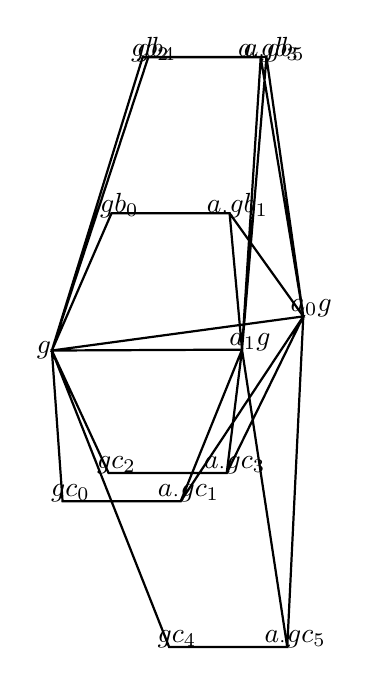
\begin{tikzpicture}
            \draw[thick](0,0)(0,0)  -- (0.7573585869902781, 1.742410894656945) -- (2.257358586990278, 1.742410894656945) -- (3.1932836010261725,0.43319882990656383) -- (0,0) -- (0,0)  -- (0.13593530800772835, -1.9155990981234063) -- (1.6359353080077284, -1.9155990981234063) -- (3.1932836010261725,0.43319882990656383) -- (0,0) -- 
(0,0)  -- (0.7573585869902781, 1.742410894656945) -- (2.257358586990278, 1.742410894656945) -- (3.1932836010261725,0.43319882990656383) -- (0,0) -- (0,0)  -- (0.7204804010709267, -1.5563780539935632) -- (2.220480401070927, -1.5563780539935632) -- (3.1932836010261725,0.43319882990656383) -- (0,0) -- 
(0,0)  -- (0.7573585869902781, 1.742410894656945) -- (2.257358586990278, 1.742410894656945) -- (3.1932836010261725,0.43319882990656383) -- (0,0) -- (0,0)  -- (1.48928186251678, -3.7659346992953777) -- (2.98928186251678, -3.7659346992953777) -- (3.1932836010261725,0.43319882990656383) -- (0,0) -- 
(0,0)  -- (1.152436218450279, 3.7238867270593956) -- (2.652436218450279, 3.7238867270593956) -- (3.1932836010261725,0.43319882990656383) -- (0,0) -- (0,0)  -- (0.13593530800772835, -1.9155990981234063) -- (1.6359353080077284, -1.9155990981234063) -- (3.1932836010261725,0.43319882990656383) -- (0,0) -- 
(0,0)  -- (1.152436218450279, 3.7238867270593956) -- (2.652436218450279, 3.7238867270593956) -- (3.1932836010261725,0.43319882990656383) -- (0,0) -- (0,0)  -- (0.7204804010709267, -1.5563780539935632) -- (2.220480401070927, -1.5563780539935632) -- (3.1932836010261725,0.43319882990656383) -- (0,0) -- 
(0,0)  -- (1.152436218450279, 3.7238867270593956) -- (2.652436218450279, 3.7238867270593956) -- (3.1932836010261725,0.43319882990656383) -- (0,0) -- (0,0)  -- (1.48928186251678, -3.7659346992953777) -- (2.98928186251678, -3.7659346992953777) -- (3.1932836010261725,0.43319882990656383) -- (0,0) -- 
(0,0)  -- (1.2250714320503318, 3.7266645458596797) -- (2.7250714320503318, 3.7266645458596797) -- (3.1932836010261725,0.43319882990656383) -- (0,0) -- (0,0)  -- (0.13593530800772835, -1.9155990981234063) -- (1.6359353080077284, -1.9155990981234063) -- (3.1932836010261725,0.43319882990656383) -- (0,0) -- 
(0,0)  -- (1.2250714320503318, 3.7266645458596797) -- (2.7250714320503318, 3.7266645458596797) -- (3.1932836010261725,0.43319882990656383) -- (0,0) -- (0,0)  -- (0.7204804010709267, -1.5563780539935632) -- (2.220480401070927, -1.5563780539935632) -- (3.1932836010261725,0.43319882990656383) -- (0,0) -- 
(0,0)  -- (1.2250714320503318, 3.7266645458596797) -- (2.7250714320503318, 3.7266645458596797) -- (3.1932836010261725,0.43319882990656383) -- (0,0) -- (0,0)  -- (1.48928186251678, -3.7659346992953777) -- (2.98928186251678, -3.7659346992953777) -- (3.1932836010261725,0.43319882990656383) -- (0,0) -- 
(0,0)  -- (0.7573585869902781, 1.742410894656945) -- (2.257358586990278, 1.742410894656945) -- (2.4148790983708883,0.011115604095153707) -- (0,0) -- (0,0)  -- (0.13593530800772835, -1.9155990981234063) -- (1.6359353080077284, -1.9155990981234063) -- (2.4148790983708883,0.011115604095153707) -- (0,0) -- 
(0,0)  -- (0.7573585869902781, 1.742410894656945) -- (2.257358586990278, 1.742410894656945) -- (2.4148790983708883,0.011115604095153707) -- (0,0) -- (0,0)  -- (0.7204804010709267, -1.5563780539935632) -- (2.220480401070927, -1.5563780539935632) -- (2.4148790983708883,0.011115604095153707) -- (0,0) -- 
(0,0)  -- (0.7573585869902781, 1.742410894656945) -- (2.257358586990278, 1.742410894656945) -- (2.4148790983708883,0.011115604095153707) -- (0,0) -- (0,0)  -- (1.48928186251678, -3.7659346992953777) -- (2.98928186251678, -3.7659346992953777) -- (2.4148790983708883,0.011115604095153707) -- (0,0) -- 
(0,0)  -- (1.152436218450279, 3.7238867270593956) -- (2.652436218450279, 3.7238867270593956) -- (2.4148790983708883,0.011115604095153707) -- (0,0) -- (0,0)  -- (0.13593530800772835, -1.9155990981234063) -- (1.6359353080077284, -1.9155990981234063) -- (2.4148790983708883,0.011115604095153707) -- (0,0) -- 
(0,0)  -- (1.152436218450279, 3.7238867270593956) -- (2.652436218450279, 3.7238867270593956) -- (2.4148790983708883,0.011115604095153707) -- (0,0) -- (0,0)  -- (0.7204804010709267, -1.5563780539935632) -- (2.220480401070927, -1.5563780539935632) -- (2.4148790983708883,0.011115604095153707) -- (0,0) -- 
(0,0)  -- (1.152436218450279, 3.7238867270593956) -- (2.652436218450279, 3.7238867270593956) -- (2.4148790983708883,0.011115604095153707) -- (0,0) -- (0,0)  -- (1.48928186251678, -3.7659346992953777) -- (2.98928186251678, -3.7659346992953777) -- (2.4148790983708883,0.011115604095153707) -- (0,0) -- 
(0,0)  -- (1.2250714320503318, 3.7266645458596797) -- (2.7250714320503318, 3.7266645458596797) -- (2.4148790983708883,0.011115604095153707) -- (0,0) -- (0,0)  -- (0.13593530800772835, -1.9155990981234063) -- (1.6359353080077284, -1.9155990981234063) -- (2.4148790983708883,0.011115604095153707) -- (0,0) -- 
(0,0)  -- (1.2250714320503318, 3.7266645458596797) -- (2.7250714320503318, 3.7266645458596797) -- (2.4148790983708883,0.011115604095153707) -- (0,0) -- (0,0)  -- (0.7204804010709267, -1.5563780539935632) -- (2.220480401070927, -1.5563780539935632) -- (2.4148790983708883,0.011115604095153707) -- (0,0) -- 
(0,0)  -- (1.2250714320503318, 3.7266645458596797) -- (2.7250714320503318, 3.7266645458596797) -- (2.4148790983708883,0.011115604095153707) -- (0,0) -- (0,0)  -- (1.48928186251678, -3.7659346992953777) -- (2.98928186251678, -3.7659346992953777) -- (2.4148790983708883,0.011115604095153707) -- (0,0) -- 
(0,0);
\node at (-0.1,0) {$ g $};
\node at (3.2932836010261726,0.5331988299065639) {$ a_{ 0 }g $};
\node at (2.5148790983708884,0.11111560409515371) {$ a_{ 1 }g $};
\node at (0.8573585869902781,1.842410894656945) {$ gb_{ 0 } $};
\node at (2.3573585869902782,1.842410894656945) {$ a_{\cdot} gb_{ 1 } $};
\node at (1.252436218450279,3.8238867270593957) {$ gb_{ 2 } $};
\node at (2.752436218450279,3.8238867270593957) {$ a_{\cdot} gb_{ 3 } $};
\node at (1.3250714320503318,3.8266645458596797) {$ gb_{ 4 } $};
\node at (2.825071432050332,3.8266645458596797) {$ a_{\cdot} gb_{ 5 } $};
\node at (0.23593530800772836,-1.8155990981234063) {$ gc_{ 0 } $};
\node at (1.7359353080077284,-1.8155990981234063) {$ a_{\cdot} gc_{ 1 } $};
\node at (0.8204804010709267,-1.4563780539935631) {$ gc_{ 2 } $};
\node at (2.320480401070927,-1.4563780539935631) {$ a_{\cdot} gc_{ 3 } $};
\node at (1.5892818625167802,-3.6659346992953776) {$ gc_{ 4 } $};
\node at (3.08928186251678,-3.6659346992953776) {$ a_{\cdot} gc_{ 5 } $};

            \end{tikzpicture}
            \end{center}
            \caption{Square of the complex, with edges $(g,ag), (agb, gb) \in E_A,
            (g,gb), (agb, ag) \in E_B.$ \label{fig:square}
            }
            \end{figure}

\end{multicols*}
  % \printbibliography 
\end{document}


